\section{Overview}

This study aims to comprehensively evaluate and compare the performance of OpenCL and XRT APIs for data transfers between the host CPU and FPGA global memory. Our primary objectives are to: \\

\begin{enumerate}
    \item Determine if there's a significant performance difference between OpenCL and XRT APIs for data transfers.
    \item Understand how data transfer sizes affect the performance of each API.
    \item Investigate the impact of consecutive READ/WRITE operations on transfer speeds.
    \item Identify scenarios where one API might be preferable over the other.
\end{enumerate}

To achieve these goals, we will conduct a series of benchmarks that measure: \\
\begin{enumerate}
    \item READ and WRITE speeds from CPU to global memory using both APIs.
    \item Performance of consecutive read and write operations.
    \item Transfer speeds across a wide range of data sizes, from very small to very large, incrementing by powers of 2.
\end{enumerate}

\begin{figure}[H]
    \centering
    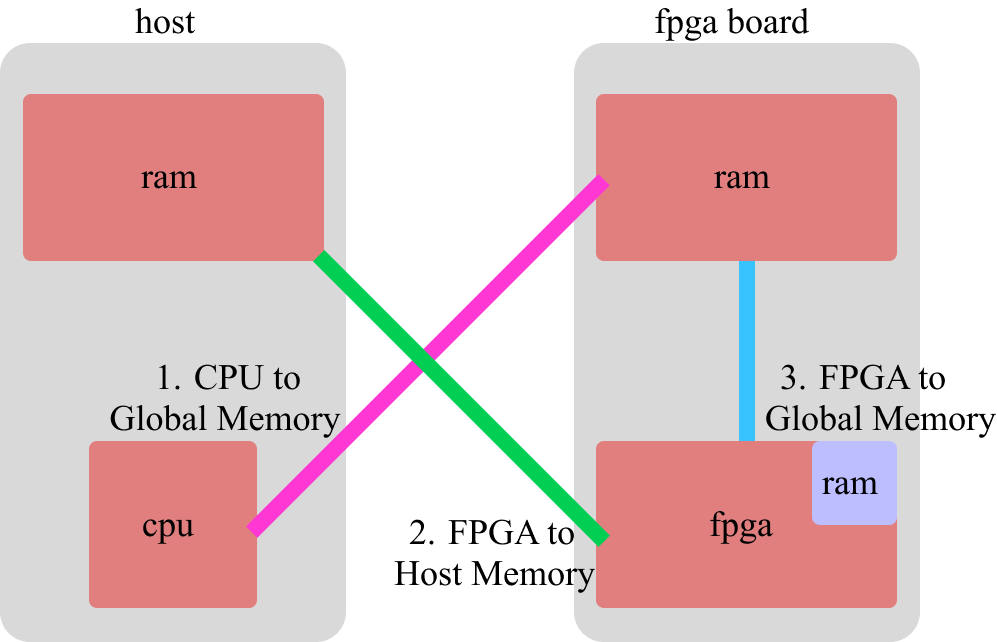
\includegraphics[width=0.6\linewidth]{content/cpu_fpga_board_layout.png}
    \caption{Layout of the Host and FPGA Board and Data Transfer Paths.}
    \label{fig:enter-label}
\end{figure}

There are 3 main ways to transfer data, referencing Fig. 1. 
\begin{enumerate}
    \item CPU READ/WRITE Global Memory

    One main way to transfer data to and from the FPGA is through the global memory (gmem). In this case, the Host will take data from it's own memory and allocate space and copy it over to the gmem. To perform this transfer, you can either use the OpenCL or XRT API. This test is used to discover whether one API has a data transfer speed advantage over the other, if at all any.

    \item FPGA READ/WRITE Global Memory - \texttt{NOT CURRENTLY SUPPORTED}

    In order for the FPGA to communicate with the Host using the previous method, it needs to read and write to the gmem. This tests is mainly used to benchmark the access speeds of the FPGA to the gmem.
    
    \item FPGA READ/WRITE Host Memory - \texttt{NOT CURRENTLY SUPPORTED}

    Another method for the Host and the FPGA to communicate is to have the FPGA read and write directly to the Host memory. This method is simpler as it removes the need to synchronise the read and writes of the Host and FPGA like in the first method. By comparing the data transfer speeds of this method to that of the total of the Host to gmem and FPGA to gmem speeds, the optimal method of data transfers can be found. \\
\end{enumerate}

We will analyze the results to identify performance trends, peak transfer rates, and any potential bottlenecks or overhead issues. This analysis will provide valuable insights for developers working on FPGA-accelerated applications, helping them make informed decisions about which API to use based on their specific use cases and data transfer requirements.

The initial platform that this was tested on \texttt{Alveo U200}, supported this feature. However, the FPGA board that AWS F1 instances use \texttt{Xilinx UltraScale Plus FPGA} was not compatible with test including the FPGA. Alternative methods are currently being investigated. \\